\section{Ratcheted Key Exchange}
\label{sec:rke}

We have seen plenty forward secure key exchange protocols in the previous chapters, but there is another security guarantee that is desirable in practice:
Post-compromise security~(PCS), which is the ability to recover from a compromise.
We adapt Figure~\ref{fig:fs:sketch}, which showed the idea of forward security, to show the idea of a protocol that provides both forward and post compromise security (Figure~\ref{fig:rke:pcs_fs_overview}).

\begin{figure}[!ht]
    \centering
    % !TeX root = ..\..\main.tex
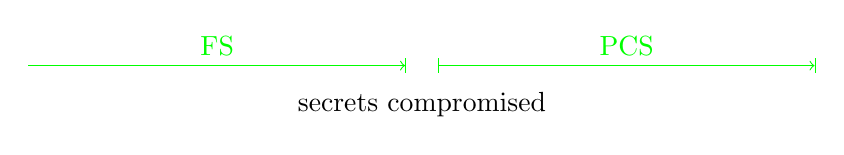
\begin{tikzpicture}%
    \draw [green, ->|] (0,0) -- (4.8,0) node [midway, above] {FS}; %FS arrow
    \node at (5,0) {\color{red}\LARGE\Lightning}; % Corruption
    \node at (5,-.5) {secrets compromised}; 
    \draw [green, |->|] (5.2,0) -- (10,0) node [midway, above] {PCS}; % PCS arrow
\end{tikzpicture}%
    \caption{A sketch of forward and post compromise security.}
    \label{fig:rke:pcs_fs_overview}
\end{figure}

A way to achieve post compromise security are the so-called Ratcheted Key Exchange protocols~(RKE).
In Figure~\ref{fig:rke:overview}, an abstract view on a two party RKE protocol is given.
After the initial key exchange, both parties regularly update their keys in a Ratcheted Key Exchange step.
Using the resulting key, a new message can be encrypted.

For the steps different cryptographic building blocks are used.
For example, X3DH might be used for the initial key exchange, the Signal Double Ratchet algorithm for the Ratcheted Key exchange step and AEAD for the encryption of the messages.

\begin{figure}[!ht]
    \centering
    % !TeX root = ..\..\main.tex
\begin{tikzpicture}
    %draw the cylinder and rotate it so that the "opening" is to the left
    \node[yshift=-2.5cm] (c) at (4.5, 0) [cylinder, shape border rotate=180, draw, minimum height=7cm, minimum width=5cm, anchor=shape center, name path=c1] {};
    
    %first step of ratcheted key exchange 
    \node[yshift=-.5cm] (1) at (c.north) {1. Initial Key Exchange};
    %draw both key derivations
    \node[yshift=-.5cm, xshift=-2.5cm] (1a1) at (1) {$\substack{\downarrow\\\scriptstyle k}$};
    \node[yshift=-.5cm, xshift= 2.5cm] (1a2) at (1) {$\substack{\downarrow\\\scriptstyle k}$};
    %connect the two keys with a dashed arrow (the anchors, e.g. 1a1.30, are "border anchors" that use an angle)
    \draw[<->, dashed] (1a1.30) -- (1a2.150);
    
    %second step
    \node[yshift=-1cm] (2) at (1) {2. Ratcheted Key Exchange};
    %draw refreshing of keys
    \node[yshift=-.5cm, xshift=-2.5cm] (2a1) at (2) {$k\circlearrowleft$};
    \node[yshift=-.5cm, xshift= 2.5cm] (2a2) at (2) {$\circlearrowleft k$};

    %third step
    \node[yshift=-1cm] (3) at (2) {3. Secure Channel};
    %first channel cylinder below the third step (anchor is "shape center", since the normal "center" uses the actual height of the 3d cylinder)
    \node[yshift=-.5cm, anchor=shape center] (3Channel1) at (3) [cylinder, shape border rotate=180, draw, minimum height=5.2cm, minimum width=.5cm] {};
    %draw refreshing keys
    \node[yshift=-.5cm, xshift=-2.5cm] (3a1) at (3Channel1) {$k\circlearrowleft$};
    \node[yshift=-.5cm, xshift= 2.5cm] (3a2) at (3Channel1) {$\circlearrowleft k$};
    %second channel cylinder (no anchor=shape center since we use the shape center anchor of the first cylinder for placement)
    \node[yshift=-1cm] (3Channel2) at (3Channel1) [cylinder, shape border rotate=180, draw, minimum height=5.2cm, minimum width=.5cm] {};

    %arrows from the keys in the second step to the first channel in the third step
    \draw [->] (2a1) -- (3Channel1.after top);
    \draw [->] (2a2) -- (3Channel1.before bottom);


    %ALICE and BOB
    \node (A) at (0, 0) {\textbf{Alice}};
    \node (B) at (9, 0) {\textbf{Bob}};

    %the two messages send from Alice
    \node (A_m1) at (0, -3) {$m$};
    \node (A_m2) at (0, -4) {$m$};

    %draw the arrow connecting the first message and the first channel
    %this path is used to get the intersection
    \path[name path=A_m1path] (A_m1) -- (3Channel1.top);
    %calculate the intersections (they are named A_m1_intersect-1, A_m1_intersect-2, ...) and draw the black part of the arrow
    \draw[-,name intersections={of=c1 and A_m1path, name=A_m1_intersect}] (A_m1) -- (A_m1_intersect-1);
    %draw the gray part of the arrow
    \draw[->, gray] (A_m1_intersect-1) -- (3Channel1.top);

    %draw the arrow connecting the second message and the second channel
    \path[name path=A_m2path] (A_m2) -- (3Channel2.top);
    \draw[<-,name intersections={of=c1 and A_m2path, name=A_m2_intersect}] (A_m2) -- (A_m2_intersect-1);
    \draw[-, gray] (A_m2_intersect-1) -- (3Channel2.top);

    %the messages bob receives
    \node (B_m1) at (9, -3) {$m$};
    \node (B_m2) at (9, -4) {$m$};

    %arrows connecting the first channel to bobs first message
    \path[name path=B_m1path] (B_m1) -- (3Channel1.bottom);
    %the gray and black parts of the arrow are switched
    \draw[-,,gray, name intersections={of=c1 and B_m1path, name=B_m1_intersect}] (3Channel1.bottom) -- (B_m1_intersect-1);
    \draw[->] (B_m1_intersect-1) -- (B_m1);

    %arrows connecting the second channel to bobs second message
    \path[name path=B_m2path] (B_m2) -- (3Channel2.top);
    \draw[<-, gray, name intersections={of=c1 and B_m2path, name=B_m2_intersect}] (3Channel2.bottom) -- (B_m2_intersect-1);
    \draw[-] (B_m2_intersect-1) -- (B_m2);

    %Left side FS-arrows
    \draw[->|, green] (.5, -.5) -- (.5, -1.25) node [midway,left] {FS};
    \node at (.5, -1.5) {\color{red}\Large\Lightning}; % corruption arrow
    \draw[|->|, green] (.5, -1.75) -- (.5, -3.25);
    \draw[|->, green] (.5, -3.75) -- (.5, -5);

    %Right side FS-arrows
    \draw[->|, green] (8.5, -.5) -- (8.5, -1.25);
    \draw[|->|, green] (8.5, -1.75) -- (8.5, -3.25);
    \node at (8.5, -3.5) {\color{red}\Large\Lightning}; %corruption arrow
    \draw[|->, green] (8.5, -3.75) -- (8.5, -5) node [midway, right] {PCS};

\end{tikzpicture}
    \caption{Overview of the Ratcheted Key Exchange~(RKE) protocol.}
    \label{fig:rke:overview}
\end{figure}